%!TEX root = ../thesis.tex

\section{シミュレータ}
開発が必要な項目にシミュレータがある.
AIFormulaのような人の歩行速度以上で移動するロボットは検証する場所を確保することが用意ではないため, アルゴリズムの初期検証などはシミュレータ環境で検証・改善を行うことが望ましい.
AIFormulaでは基本的な機能が実装されたシミュレータ環境が運営から提供されている.
Fig.5.1に提供されたシミュレータ環境の外観を示す.
Fig.5.2にシミュレートするモビリティとコースの外観を示す.

\begin{figure}[H]
  \centering
 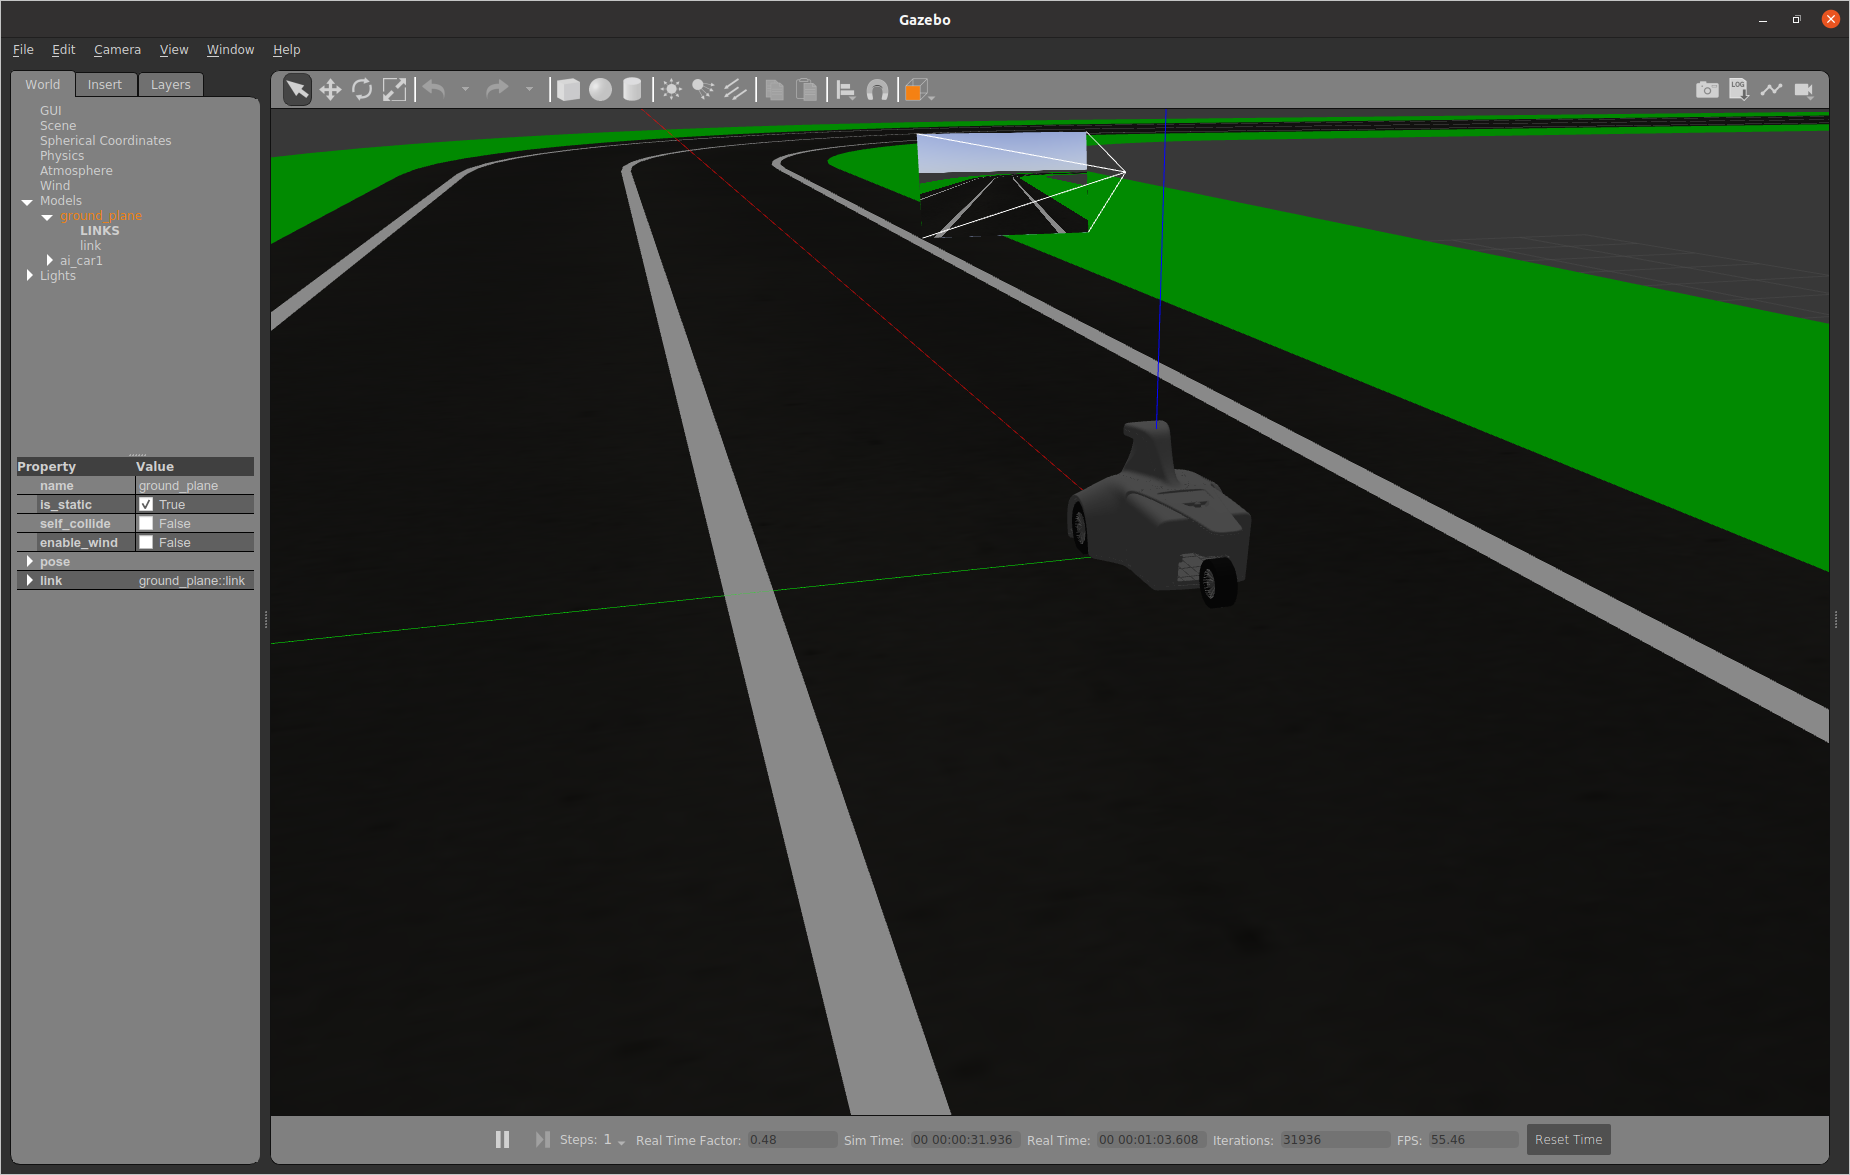
\includegraphics[keepaspectratio, scale=0.2]
      {images/simulator.png}
 \caption{Appearance of simulator}
 \label{fig:simulator}
\end{figure}

\begin{figure}[H]
  \centering
 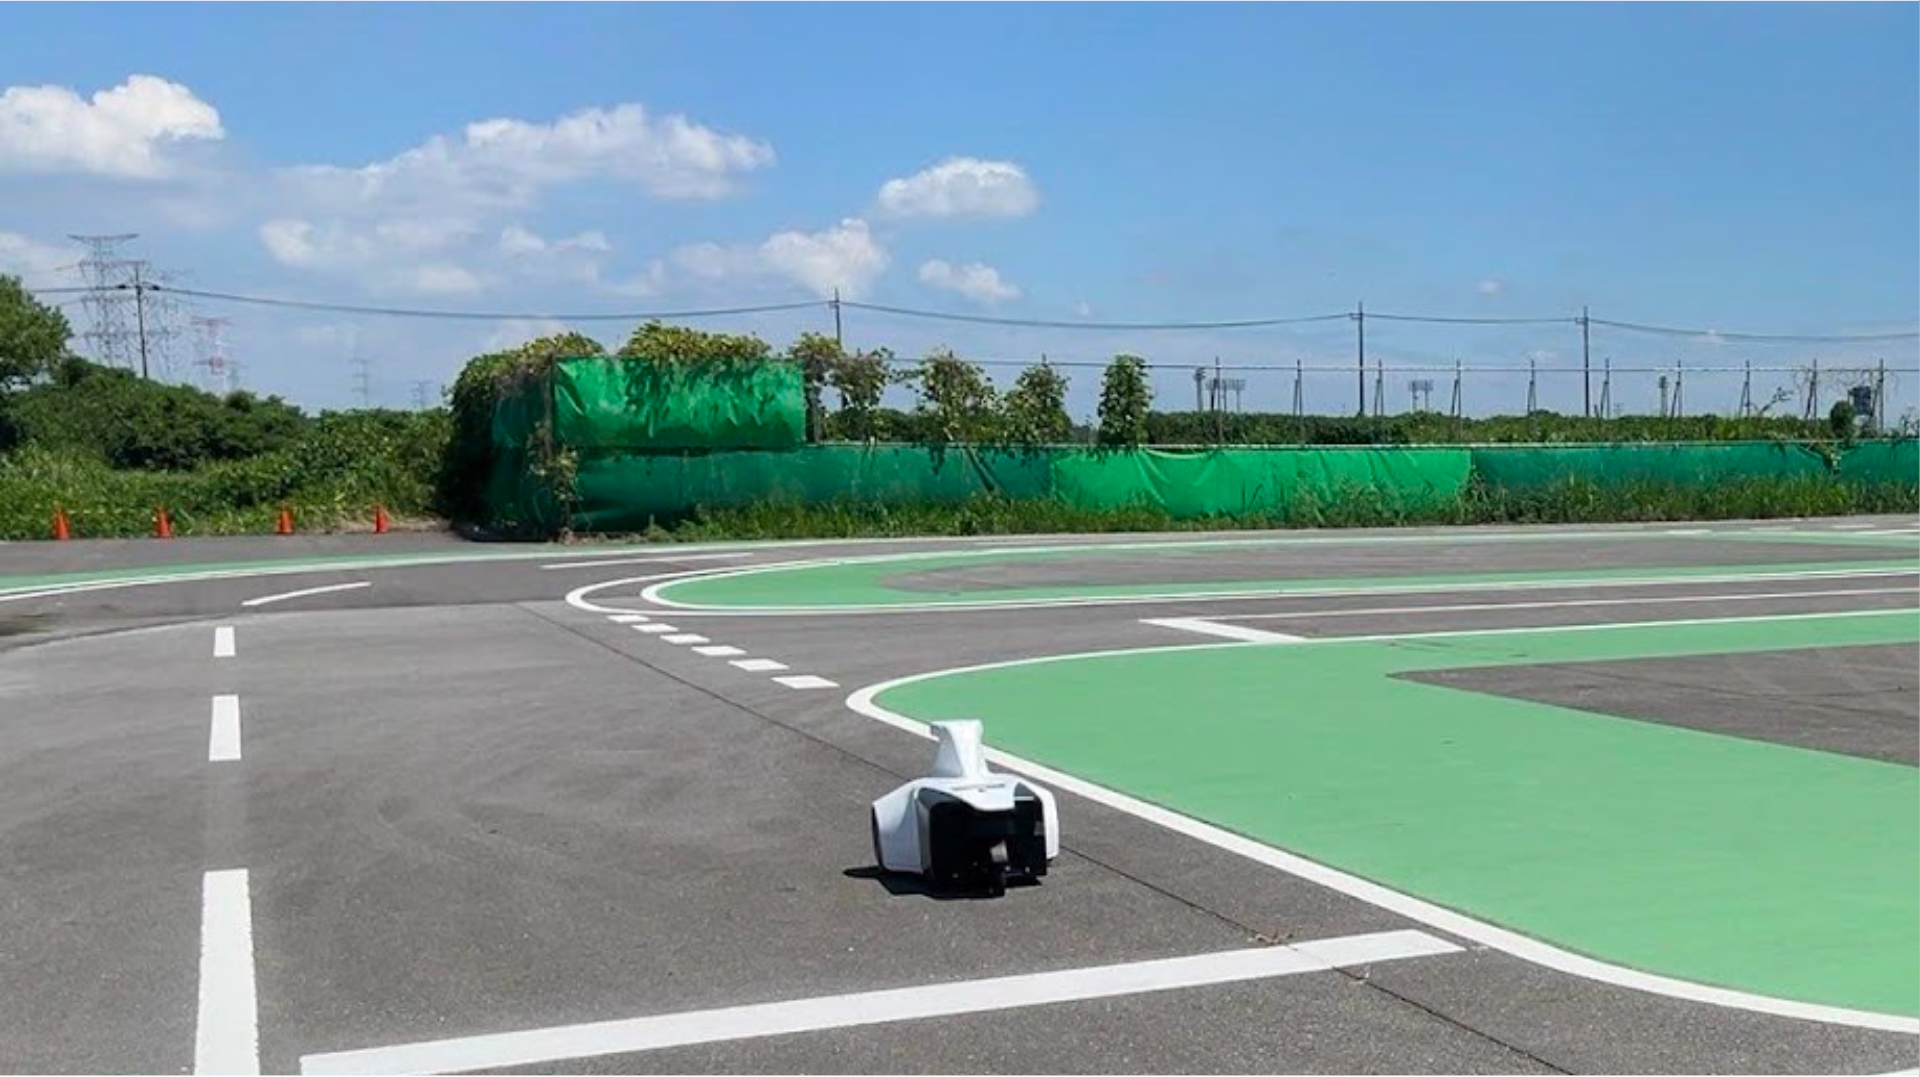
\includegraphics[keepaspectratio, scale=0.2]
      {images/realworld.png}
 \caption{AIFormula and racing course}
 \label{fig:simulator}
\end{figure}

\newpage

提供されたシミュレータ環境では基本的な機能が実装されているが, GNSS+IMUセンサ(VectorNav VN-200)の出力を再現できていない.
そのため, GNSS+IMUセンサ(VectorNav VN-200)の出力を再現する機能を追加して, 提供されたシミュレータを拡張して使用している.

シミュレータはROS 2とGazebo上で実装されており, Fig.5.3のようなノードの構成になっている.

\begin{figure}[H]
  \centering
 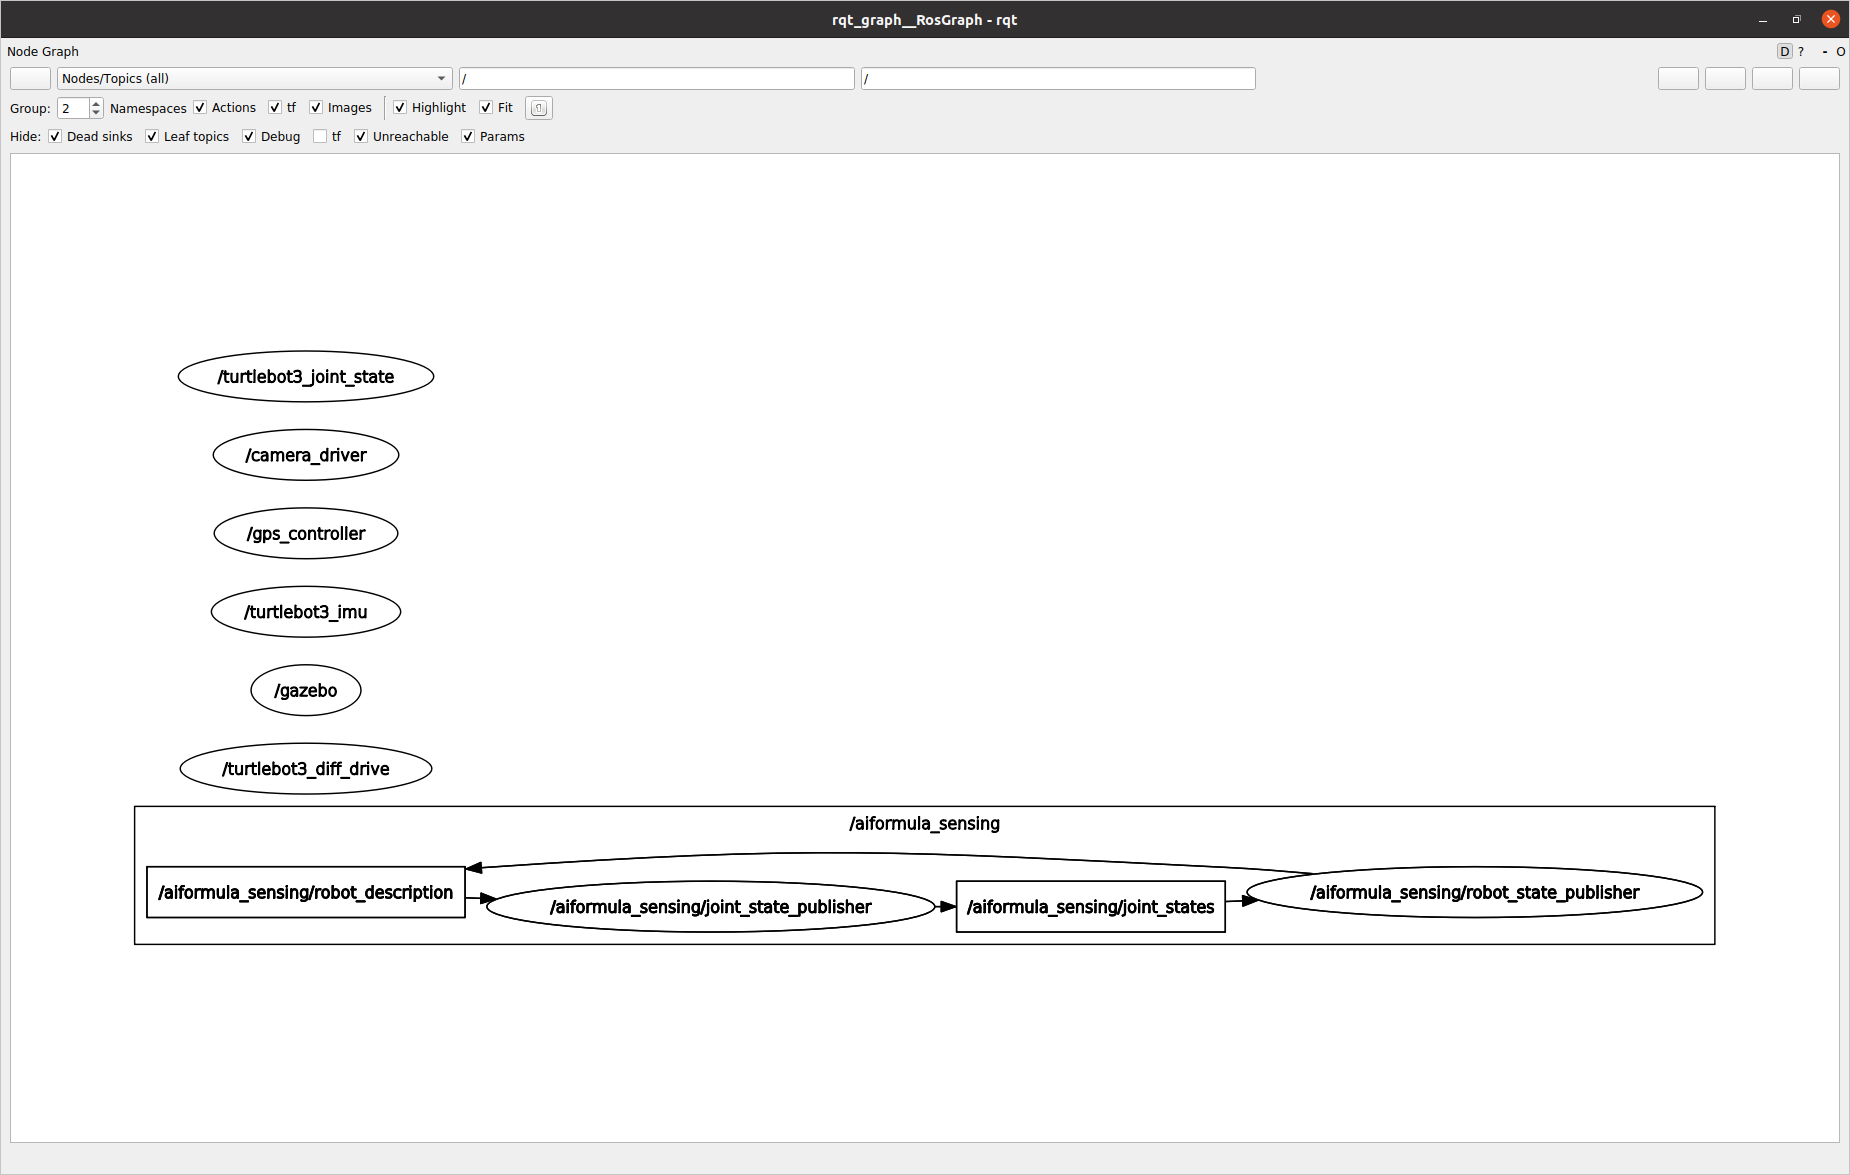
\includegraphics[keepaspectratio, scale=0.2]
      {images/rqt.png}
 \caption{Configuration of ROS 2 nodes}
 \label{fig:simulator}
\end{figure}

シミュレーションする主なセンサとアクチュエータを以下に示す.

\begin{table}[H]
  \centering
  \caption{Sensors and actuators to be simulated}
  \begin{tabular}{lclll}
  \cline{1-2}
  \multicolumn{1}{|l|}{}         & \multicolumn{1}{c|}{Camera}      &  &  &  \\
  \multicolumn{1}{|c|}{Sensor}   & \multicolumn{1}{c|}{IMU(Inertial Measurement Devices)} &  &  &  \\
  \multicolumn{1}{|l|}{}         & \multicolumn{1}{c|}{GNSS}        &  &  &  \\ \cline{1-2}
  \multicolumn{1}{|l|}{Actuator} & \multicolumn{1}{c|}{Drive motor} &  &  &  \\ \cline{1-2}
                                 & \multicolumn{1}{l}{}             &  &  & 
  % \caption{Sensors and actuators to be simulated}
  \end{tabular}
\end{table}

\section{実験の概要}
本システムではセンサはGNSS+IMU(VectorNav VN-200)を使用している.
自動で経路追従するソフトウェアを開発する際にはこれらを再現したシミュレータ環境を開発することで, オフラインで開発ができる環境を用意することができる.
用意したシミュレータ環境を使用することで開発した経路追従のアルゴリズムの追従性などを確認することができる.
そこでGNSS+IMU(VectorNav VN-200)の出力を再現したシミュレータ環境を使用して, 開発した経路追従パッケージの有効性を確認する.


\section{実験環境}
前述の提供されたシミュレータ環境にGNSS+IMUセンサ(VectorNav VN-200)の出力を追加したシミュレータ環境を使用する.
Fig.5.4にシミュレータで扱うコースの全体図を示す.
Table.5.2にシミュレータに使用するPCの仕様を示す.ソフトウェアにはROS 2 foxyを使用し, シミュレータ環境にはGazebo Classicを使用している.

\begin{figure}[H]
  \centering
 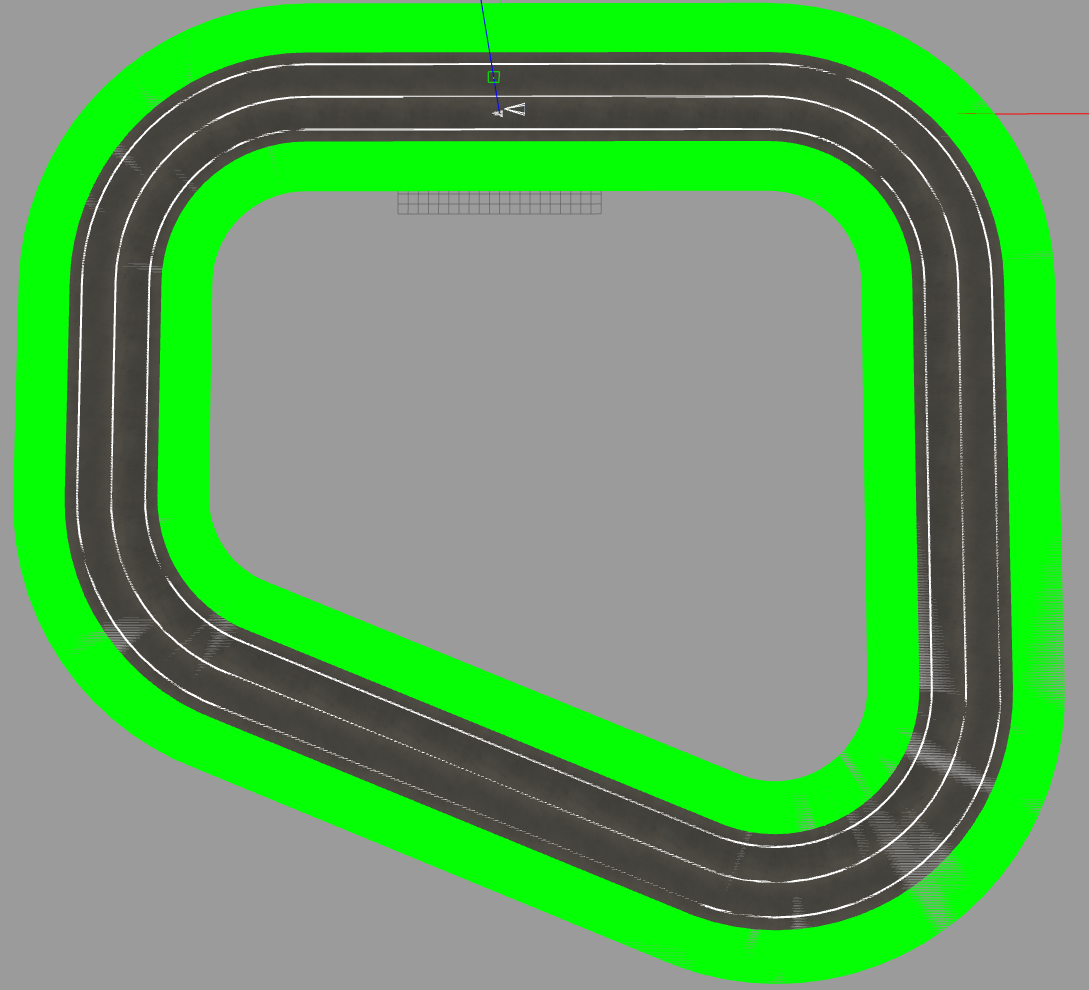
\includegraphics[keepaspectratio, scale=0.3]
      {images/topviewsim.png}
 \caption{Simulator world top view}
 \label{fig:simulator}
\end{figure}

\begin{table}[H]
  \centering
  \caption{experimental devece}
  \begin{tabular}{cclll}
  \cline{1-2}
  Computer             & Let`s note CF-SV &  &  &  \\
  OS                   & Ubuntu20.04 LTS  &  &  &  \\
  ROS 2                & Foxy             &  &  &  \\
  simulator            & Gazebo Classic   &  &  &  \\
  \multicolumn{1}{l}{} &                  &  &  &  \\
  \multicolumn{1}{l}{} &                  &  &  & 
  \end{tabular}
\end{table}

\section{実験内容}
前述のシミュレータ環境で作成した経路追従ソフトウェアを使用することによって, 作成した経路追従アルゴリズムの追従性を検証する.
本実験で走行するコースをFig.5.5に示す.
本実験では予め決めたコースを1周したときのそれぞれの評価項目を確認することで作成した経路追従アルゴリズムの追従性の確認を行う.

\begin{figure}[H]
  \centering
 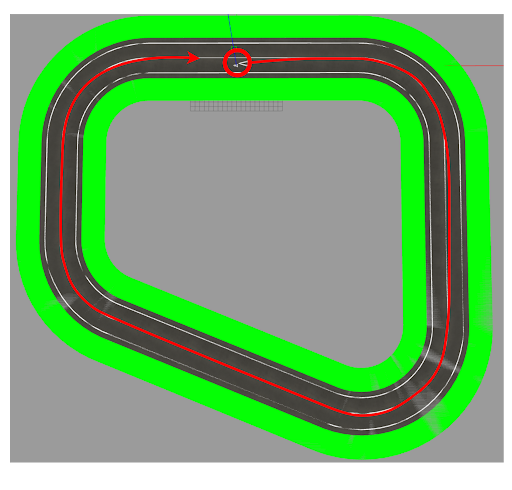
\includegraphics[keepaspectratio, scale=0.6]
      {images/simulatorpath.png}
 \caption{Simulator course}
 \label{fig:simulator}
\end{figure}

\subsection{アルゴリズムの有効性を確認する実験}
作成した経路追従アルゴリズムに追従性があるかどうか確認する実験を行う.
本実験では前述の通り予め決めたコースを1周させたときの評価項目や走行経路の軌跡から作成した経路追従アルゴリズムの有効性を判断する.

\section{実験結果}
シミュレータ環境で作成した経路追従ソフトウェアを使用することで実験を行った.

実験の様子をFig.5.6に示す.
シミュレータで自律走行したときのロボットの軌跡をFig.5.7に示す.
結果として, シミュレータ環境のコースを周回することができた.

\begin{figure}[H]
  \centering
 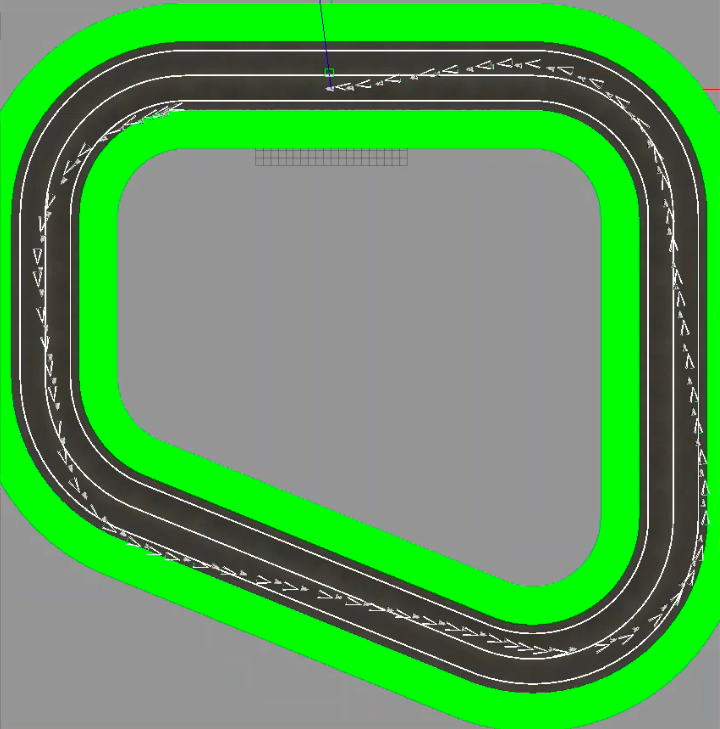
\includegraphics[keepaspectratio, scale=0.5]
      {images/simulatorfollowerpath.png}
 \caption{The AIFormula path-following behavior on the simulator}
 \label{fig:simulatorpath}
\end{figure}